\documentclass[a4paper, notitlepage, 10pt]{article}
\usepackage{geometry}
\fontfamily{times}
\geometry{verbose,tmargin=30mm,bmargin=25mm,lmargin=25mm,rmargin=25mm}
% \pagestyle{empty}
% end configs
\usepackage{setspace,relsize}               
\usepackage{moreverb}                        
\usepackage{url}
\usepackage{hyperref}
\hypersetup{colorlinks=true,citecolor=blue}
\usepackage{amsmath}
\usepackage{mathtools} 
\usepackage{amsthm}
\usepackage{amssymb}
\usepackage{indentfirst}
\usepackage{todonotes}
\usepackage[authoryear,round]{natbib}
\bibliographystyle{apalike}
\usepackage[pdftex]{lscape}
\usepackage[utf8]{inputenc}
\usepackage{subfigure}

% Title Page
\title{\vspace{-9ex}\centering \bf Uncertainty analysis of key epidemiological quantities}
\author{
Luiz Max F. de Carvalho\\
School of Applied Mathematics, Get\'ulio Vargas Foundation.
% Program for Scientific Computing (PROCC), Oswaldo Cruz Foundation.\\
% Institute of Evolutionary Biology, University of Edinburgh.\\
}
\DeclareMathOperator*{\argmin}{arg\,min}
\DeclareMathOperator*{\argmax}{arg\,max}
\newtheorem{theorem}{Theorem}[]
\newtheorem{proposition}{Proposition}[]
\newtheorem{remark}{Remark}[]
\setcounter{theorem}{0} % assign desired value to theorem counter
\begin{document}
\maketitle

\begin{abstract}
In these notes we give a few key epidemiological quantities which can be computed in closed-form for a few important ODE-based epidemic models, such as SIR and SEIR.
We also show one can use these to carry out prior predictive checks.
Key-words: Bayesian inference; mathematical epidemiology; prior predictive checks; final epidemic size; peak size. 
\end{abstract}

\section*{SIR model}

The SIR model we are interested in this note is given by the system:

\begin{eqnarray*}
\frac{dS}{dt}&=& - \beta SI,\\
\frac{dI}{dt}&=&  \beta SI - \gamma I,\\
\frac{dR}{dt}&=& \gamma I, 
\end{eqnarray*} 
where  $S(t) + I(t) + R(t) = 1 \: \forall t$, $\beta$ is the transmission (infection) rate and $\gamma$ is the recovery rate.
The basic reproductive number is 
\begin{equation}
\label{eq:r0def}
R_0 = \frac{\beta}{\gamma}. 
\end{equation}

\subsection*{Final epidemic size}

Now, we would like to know what the final epidemic size would be.
This is $\lim_{t \to \infty} R(t) := R(\infty)$, which leads to $S(\infty) = N - R(\infty)$.
To compute $S(\infty)$, first write 
\begin{equation}
 \frac{dI}{dS} = -1 + \frac{N}{R_0 S},
\end{equation}
which gives
\begin{equation}
\label{eq:I_of_t}
 I(t) = -S(t) + \frac{N}{R_0} \log S(t) + C,
\end{equation}
where $C$ can be determined from the initial conditions~\citep{Miller2012} and thus:
\begin{align}
    S(\infty)&= I(0) + S(0) + \frac{N}{R_0} \log\left(\frac{S(\infty)}{S(0)}\right)\\
    R(\infty) &= N - S(\infty)
\end{align}


Letting $a = R_0/N$ and $b = N - \log S(0)$, we arrive at the following expression for $S(\infty)$:
\begin{equation}
\label{eq:Rinfty}
    S(\infty) = -\frac{1}{a} W\left(- a e^{-b} \right),
\end{equation}
where $W$ is the Lambert product log function.

\subsection*{Peak size}

To find the maximum value of $I(t)$, i.e., the peak size, $I_{\max}$, we need to solve $\frac{dI}{dt} = 0$:
\begin{equation}
 I(\beta S - \gamma) = 0 \implies \bar{S} = \frac{1}{R_0}.
\end{equation}
Plugging $\bar{S}$ into equation~(\ref{eq:I_of_t}) gives
\begin{align}
\label{eq:Imax}
    I_{\max} &= S(0) + I(0)-\frac{1}{R_0} \log S(0) - \frac{1}{R_0} + \frac{1}{R_0} \log \frac{1}{R_0},\\
%     &= S_0 + I_0 -\frac{\log S_0 + \log R_0  + 1 }{R_0}.\\
    &= S(0) + I(0) - \frac{1}{R_0} \left[1 + \ln(S(0)R_0)\right].
\end{align}

Making the approximation $S(0) + I(0) \approx S(0) \approx N$, we get
\begin{equation}
 \label{eq:approx_Imax}
I_{\max} =  N - \frac{\log R_0 + 1}{R_0}, 
\end{equation}
for the number of individuals that are infectious at the peak.

\section*{SEIR model}

For the SEIR model the system is
\begin{eqnarray*}
\frac{dS}{dt}&=& -\beta S (I +\epsilon E),\\
\frac{dE}{dt}&=& \beta S (I +\epsilon E) - \kappa E,\\
\frac{dI}{dt}&=& \kappa E - \alpha I,\\
\frac{dR}{dt}&=& \alpha I, 
\end{eqnarray*} 
with $S(0) = S_0$, $E(0) = E_0$, $I(0) = R(0) = 0$ and $S(t) + E(t) + I(t) + R(t) = N$.

Under this model $S(\infty)$ can be calculated using the expression in~(\ref{eq:Rinfty}) by writing making
\begin{align}
 &b  = R_0 - \log S(0) -\frac{\epsilon\beta}{N}(N-S(0)),\\  &R_0 = \frac{\beta N}{\gamma} + \frac{\beta N\epsilon}{\kappa} = \beta N \left( \frac{\kappa + \gamma\epsilon}{\gamma\kappa}\right).
%   \beta N \left( \frac{1}{\gamma} + \frac{\epsilon}{\kappa}\right)
\end{align}

The peak size for the SEIR model can be computed if we consider infectious and exposed individuals jointly~\citep{Feng2007} by writing $Y(t) = E(t) + I(t)$.
We can then proceed analogously to the case of the SIR model and arrive at 
\begin{equation}
 \label{eq:Ymax}
 Y_{\max} = S(0) + Y(0) - \frac{1}{R_0} \left[1 + \ln(S(0)R_0)\right].
\end{equation}

\section*{Uncertainty analysis}

In the context of a (Bayesian) statistical analysis of deterministic epidemic models, some or all of the parameters, $\theta$, are unknown and we want to estimate them from data.
Assuming we can represent uncertainty about the parameters as a joint probability distribution $\pi(\theta)$, we can then ask what the distribution on the quantity of interest (q.o.i.) such as $R_0$, $R(\infty)$ or $I_{\max}$ induced by $\pi(\theta)$.
Let $\varphi(\theta)$ be the q.o.i.
The predictive check procedure can be summarised as follows.
For a number $M \in \mathbb{N}$ of iterations, do for $i = 1, \ldots, M$:
\begin{enumerate}
 \item Draw $\theta^{(i)} \sim \pi(\cdot)$;
 \item Compute $\varphi^{(i)} = \varphi(\theta^{(i)})$.
\end{enumerate}
The distribution $\pi(\varphi(\theta))|J|$ can then be approximated from the samples $\boldsymbol\varphi$.

As a first illustration of this procedure, we place a prior directly on $R_0$, i.e., we interpret the basic reproductive number as a parameter rather than a derived quantity from the parameters.
We take COVID-19 as a basis and elicit Gamma and log-normal distributions with mean $2.5$ and standard deviation $0.65$ (shown in Figure~\ref{fig:simple_Imax_COVID}b).
The resulting distribution on $I_{\max}$ is shown in Figure~\ref{fig:simple_Imax_COVID}c.

\begin{figure}[!ht]
\centering
\subfigure[$I_{\max}$ as a function of $R_0$.]{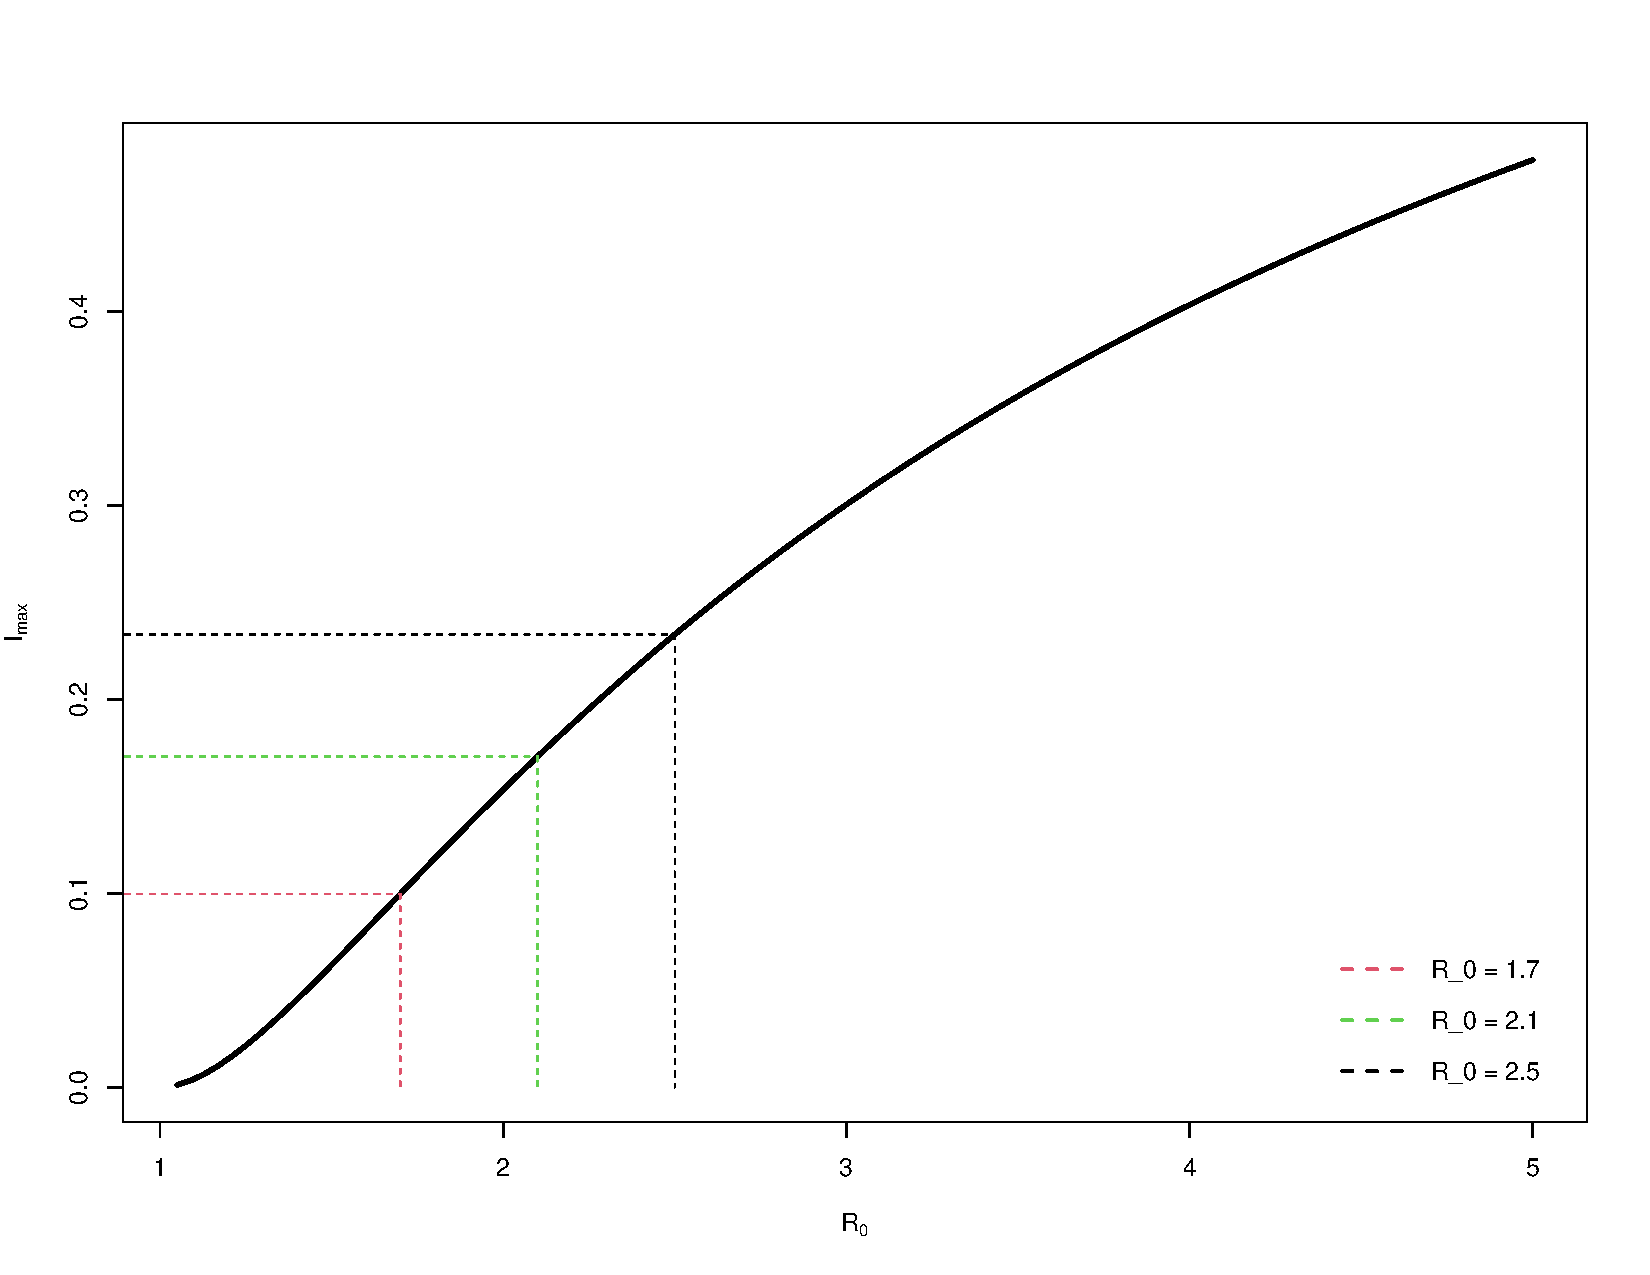
\includegraphics[scale=0.3]{../figures/Imax_vs_R0.pdf}}\\
\subfigure[Priors for $R_0$.]{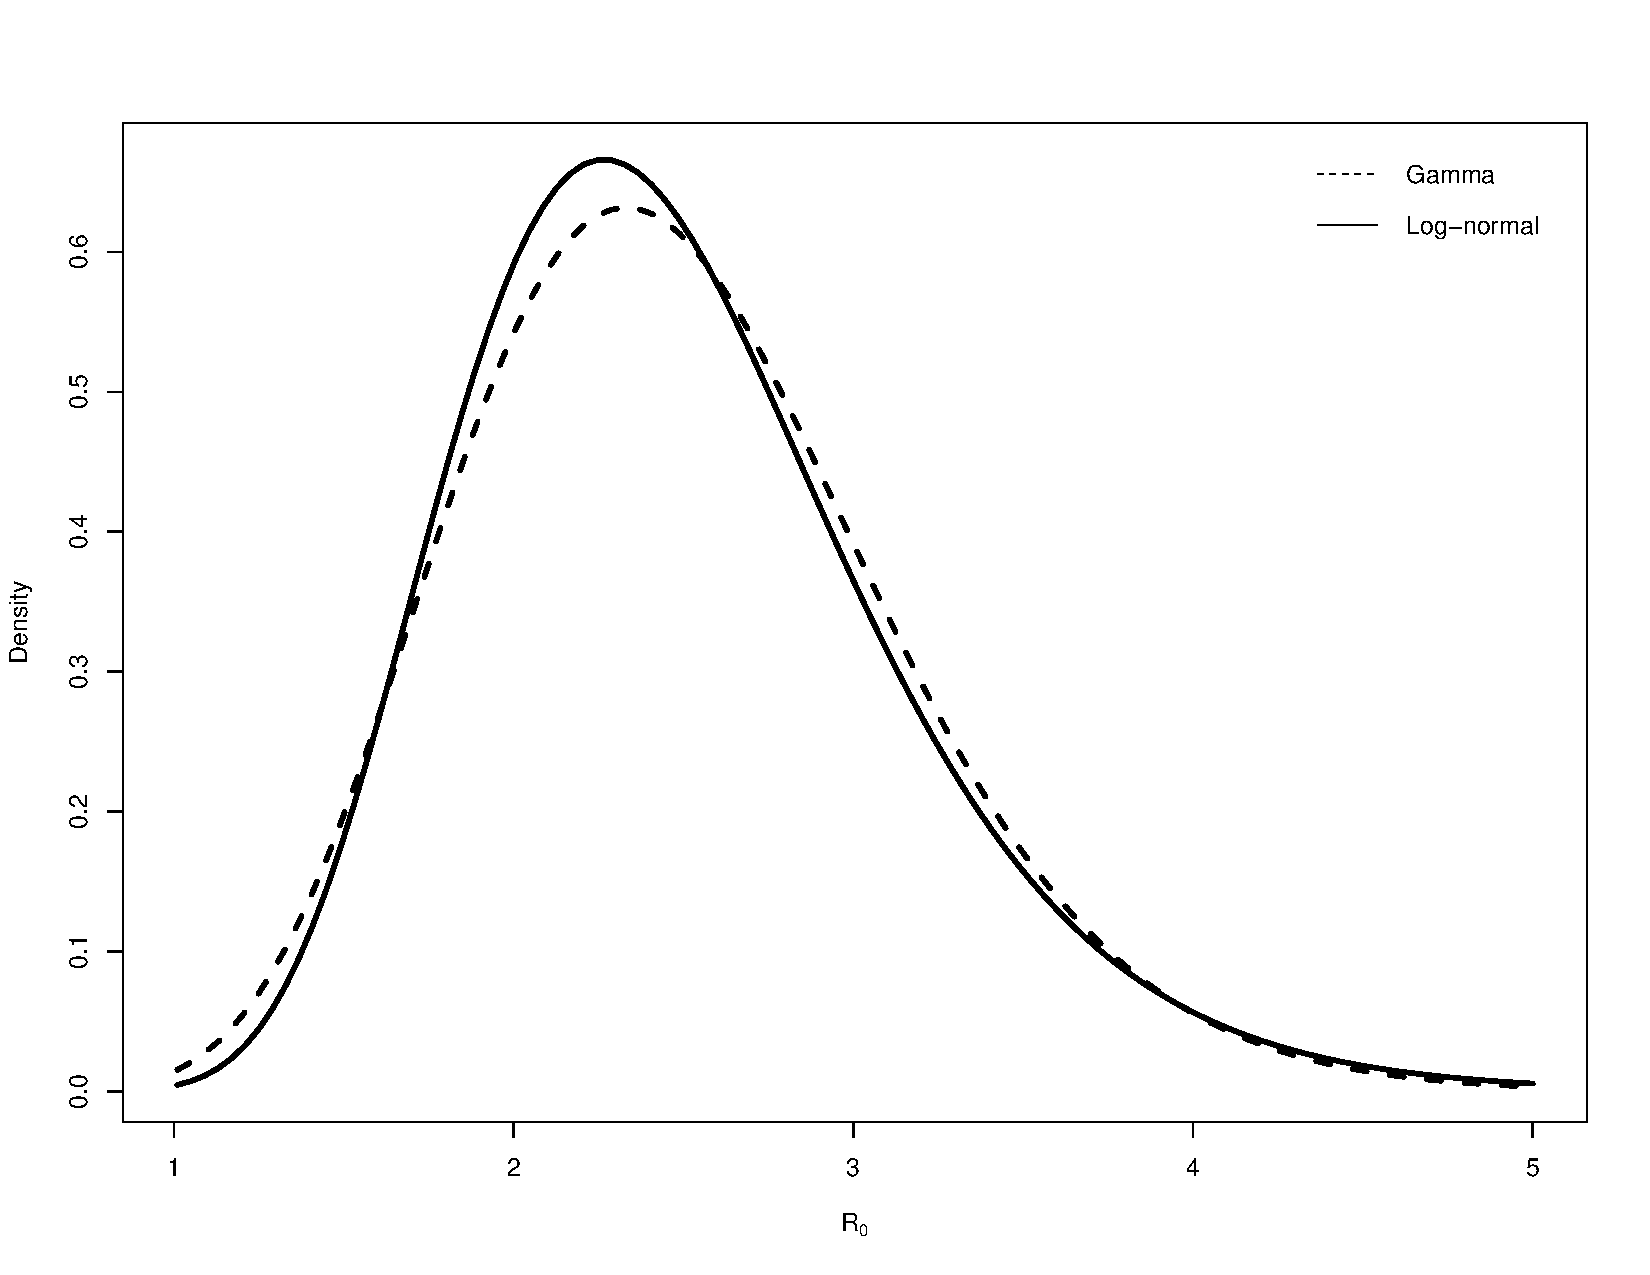
\includegraphics[scale=0.3]{../figures/priors_R0_COVID19.pdf}}\\
\subfigure[Induced distributions for $I_{\max}$.]{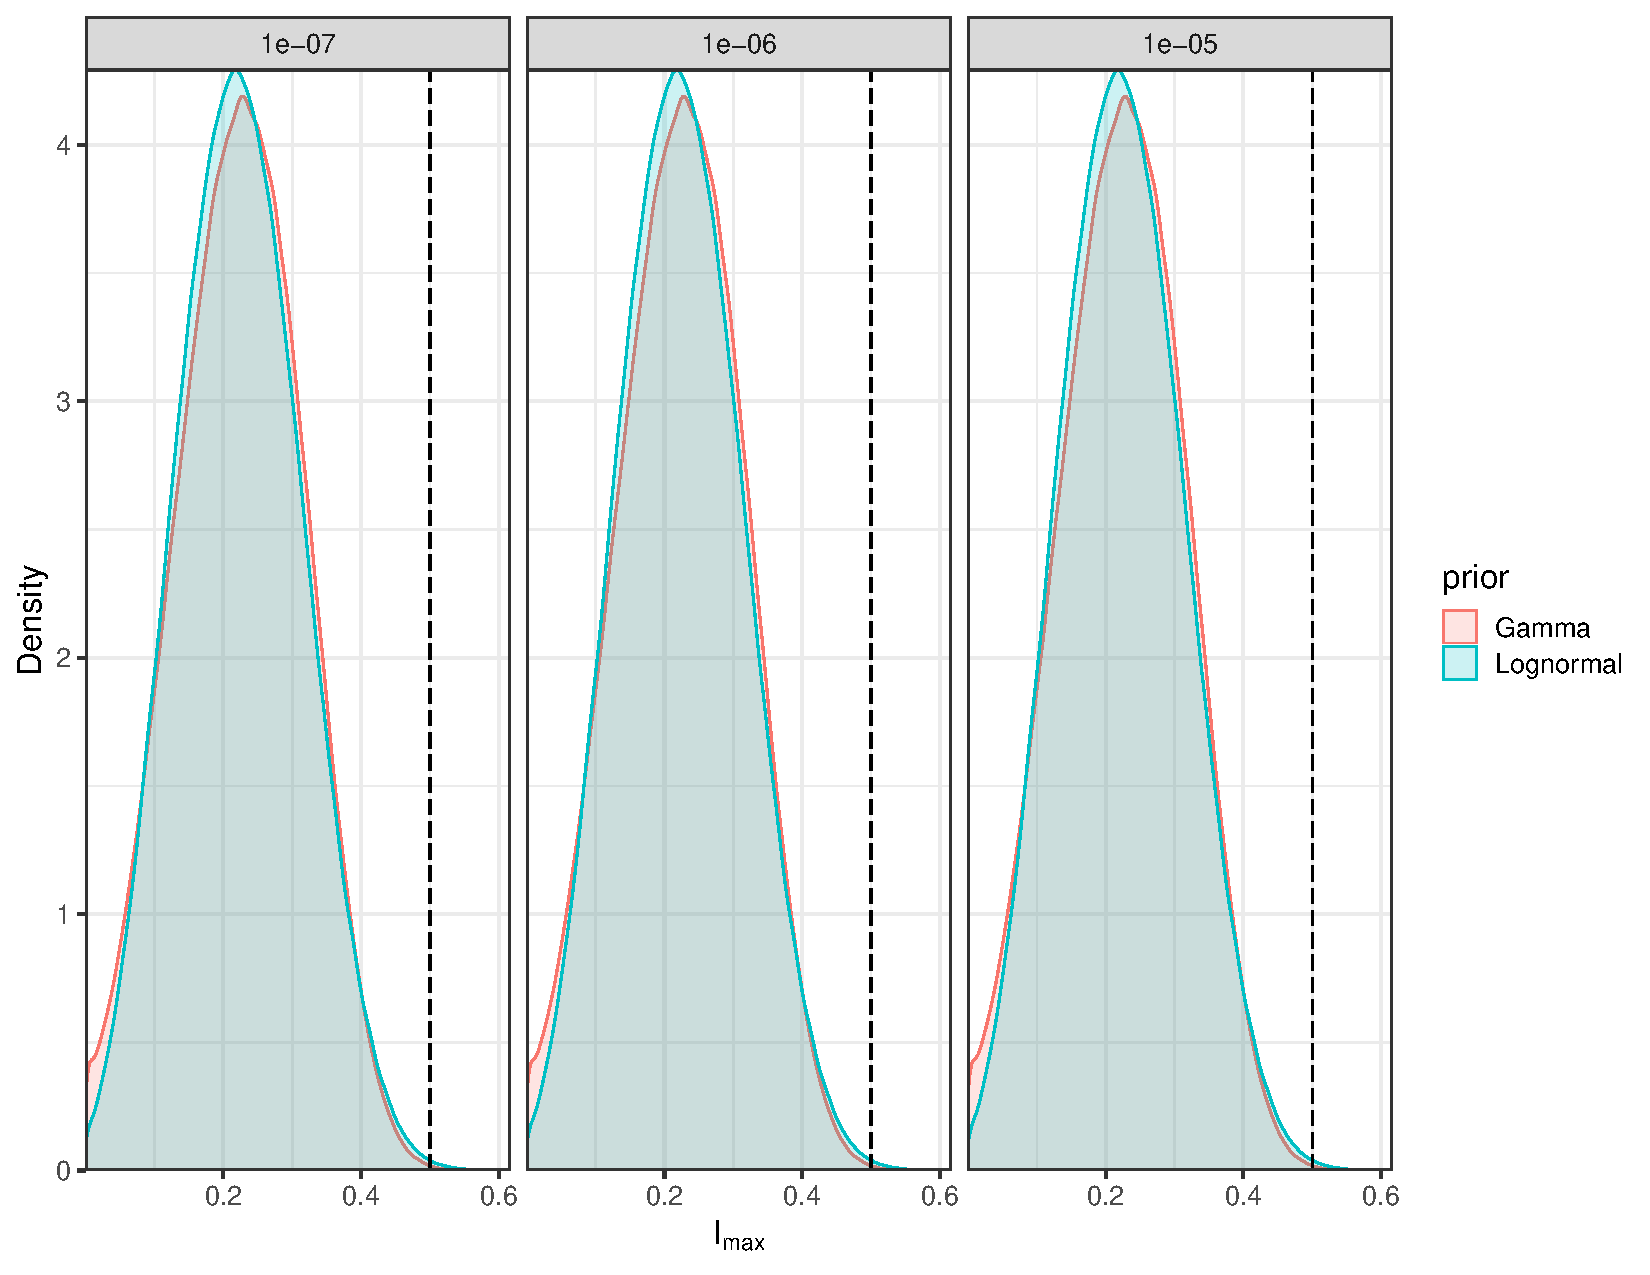
\includegraphics[scale=0.3]{../figures/Imax_COVID19_simple.pdf}}
\caption{\textbf{Uncertainty analysis of the peak size for the SIR model, priors on $R_0$}.
In panel A we show the peak size $I_{\max}$ as function of the reproductive number $R_0$.
In panel B we show two priors for $R_0$ and panel C shows the induced distributions on $I_{\max}$ for three values of $I(0)$: $10^{-7}$, $10^{-6}$, $10^{-5}$.
Vertical dashed line shows $I_{\max} = 1/2$.
In this example, $N = 1$, i.e. the system is normalised.
}
\label{fig:simple_Imax_COVID}
\end{figure}

As a second example, we consider a similar setting, by choose to place priors on $\beta$ and $\gamma$.
As with the previous analysis, we elicit Gamma and log-normal priors on the parameters.
We follow Grinsztajn et al\footnote{Case study available at~\url{https://mc-stan.org/users/documentation/case-studies/boarding_school_case_study.html}.} and set $E[\beta] = 2$ and $\operatorname{Var}(\beta) = 1$ and $E[\gamma] = 0.4$ and $\operatorname{Var}(\gamma) = 0.25$.
We show the resulting densities for $\beta$ and $\gamma$ in Figure~\ref{fig:simple_Imax_Boarding}a and b, respectively.
The resulting distribution on $I_{\max}$ is shown in Figure~\ref{fig:simple_Imax_Boarding}c, and indicates that these priors, which seem reasonable, lead to a very wide prior on $I_{\max}$  -- also on $R_0$, not shown here.

\begin{figure}[!ht]
\centering
\subfigure[$\pi(\beta)$]{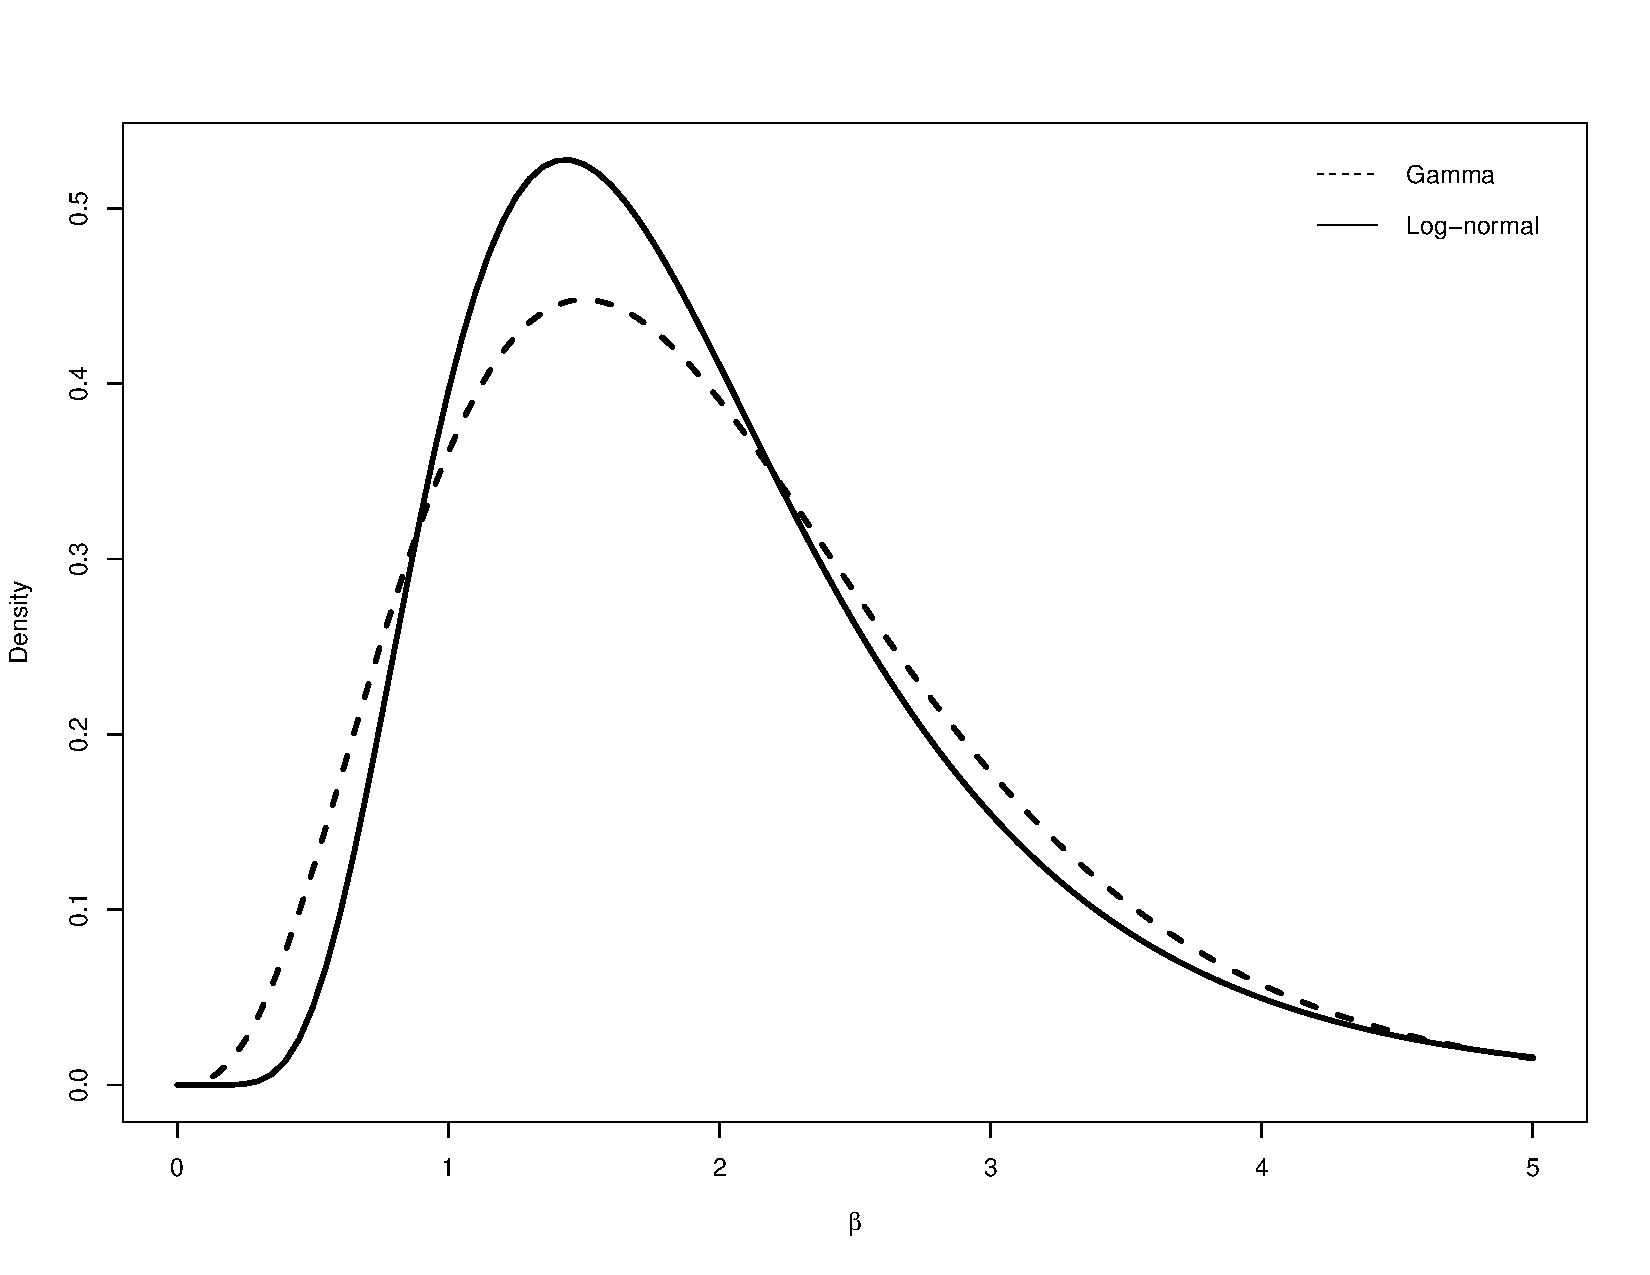
\includegraphics[scale=0.3]{../figures/caseStudyPriorBeta.pdf}}\\
\subfigure[$\pi(\gamma)$.]{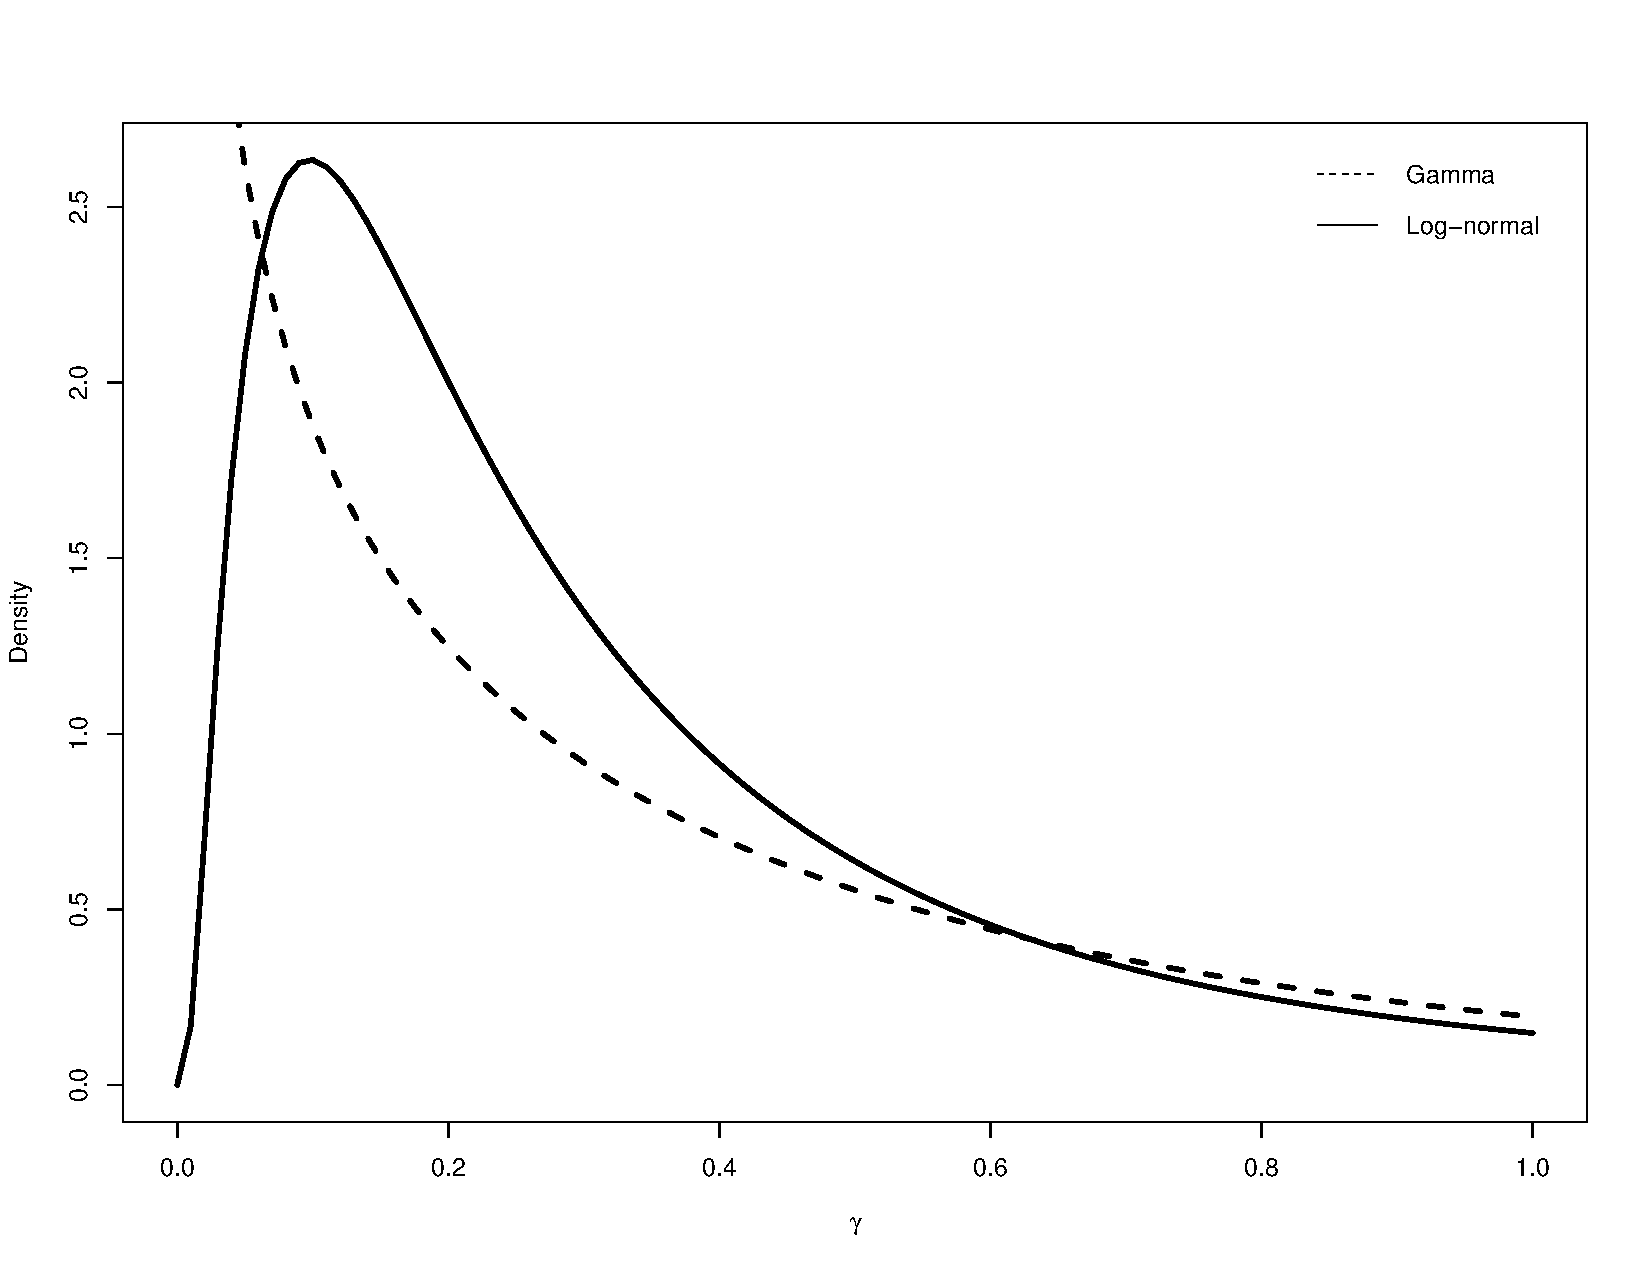
\includegraphics[scale=0.3]{../figures/caseStudyPriorGamma.pdf}}\\
\subfigure[Induced distributions for $I_{\max}$.]{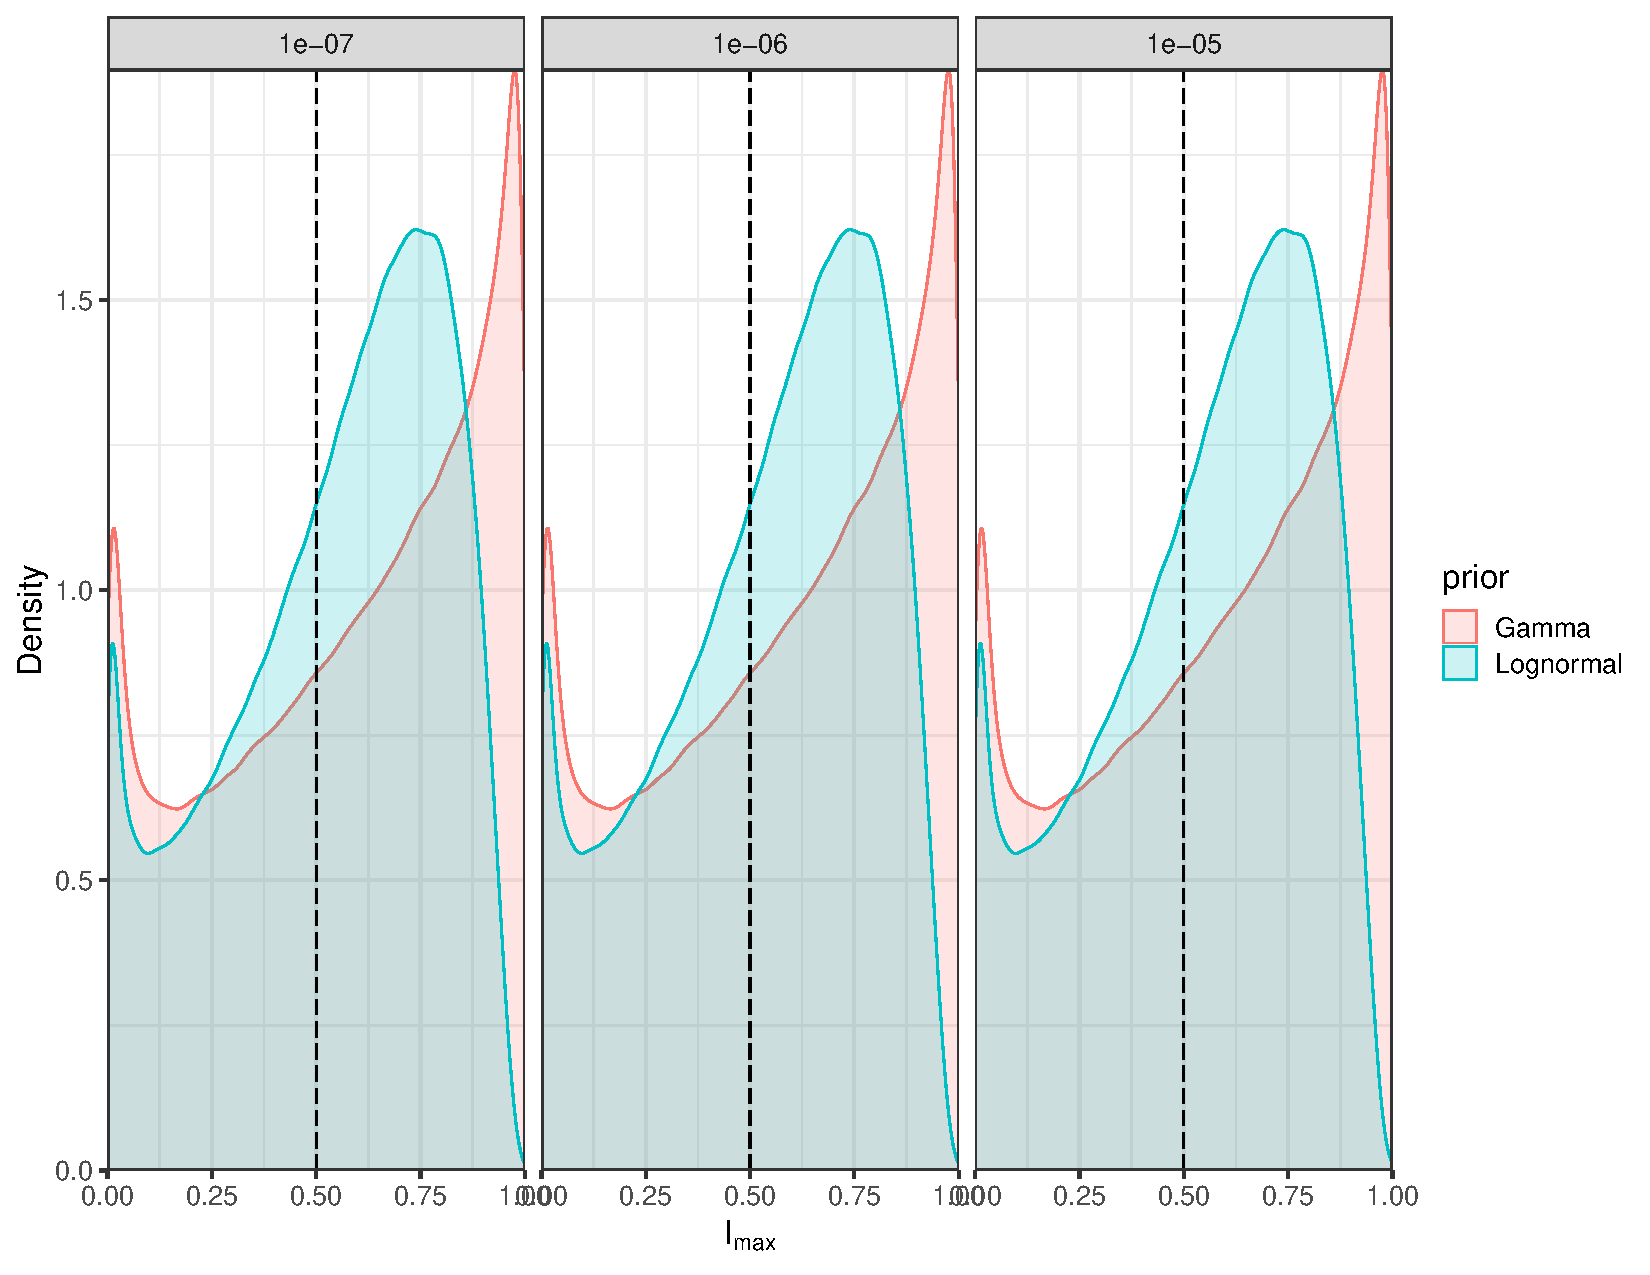
\includegraphics[scale=0.3]{../figures/Imax_priorsOnRates.pdf}}
\caption{\textbf{Uncertainty analysis of the peak size for the SIR model, priors on $\beta$ and $\gamma$}.
Panels A and B show prior distributions on $\beta$ and $\gamma$, respectively.
In panel C we show the induced distributions on $I_{\max}$ for three values of $I(0)$: $10^{-7}$, $10^{-6}$, $10^{-5}$.
Vertical dashed line shows $I_{\max} = 1/2$.
In this example, $N = 1$, i.e. the system is normalised.
}
\label{fig:simple_Imax_Boarding}
\end{figure}



\section*{Acknowledgements}

LMC would like to thank Charles Margossian (Columbia) for stimulating discussions that prompted him to write these notes in hopes these analyses become common place in statistical applications of epidemic models.

\bibliography{../R0.bib}

% \begin{figure}[!ht]
% \centering
% \includegraphics[width=\textwidth, height = 15cm]{figures/}
% \caption{\textbf{}.
% }
% \label{fig:}
% \end{figure}
\end{document}          
